\documentclass[../Report.tex]{subfiles}
\usepackage[italian]{babel}
\graphicspath{ {../../Images/} }

\begin{document}
    \chapter{Proposta di design}
    Ora procediamo con la fase di design del sito Gioco.it.
    \subsubsection{Analisi degli utenti}
    \textbf{Che target di utenti è atteso?} Come è descritto durante la ricerca etnografica capitolo \ref{chapter:ricerca etnografica} ci aspettiamo principalmente due macro target di utenti:
    \begin{itemize}
        \item Bambini e ragazzi come utilizzatori del sito (giocatori)
        \item Adulti come supervisori degli utilizzatori 
    \end{itemize}

    Il sito dovrà quindi prendere in carico le differenti richieste di entrambi i soggetti: la voglia di divertirsi dei giocatori e la propensione all'educazione e alla sicurezza da parte dei supervisori.\\
    \\
    \textbf{Perché gli utenti dovrebbero utilizzare il nostro servizio?} Perché il sito offre la più grande varietà e collezione di giochi presenti sul web e poiché sarà l'unico che offrirà un'attenzione particolare ai bisogni dei supervisori dei giocatori che giocano al sito.

    \subsubsection{Navigazione}
    \textbf{Come migliorare la navigazione tra le categorie?} Nella vecchia versione di Gioco.it alcune macro categorie non erano visibili nel menù principale e allo stesso modo c'era una grande discordanza tra le sottocategorie mostrate nella home page e quelle mostrate nel menù delle categorie e nelle categorie consigliate, sarà quindi necessario un grande lavoro di coerenza e uniformazione dei contenuti per far sì che gli utenti possano navigare correttamente nel sito.

    \subsubsection{Etica del sito}
    \textbf{I supervisori devono ancora essere preoccupati?} Al momento il sito Gioco.it non fornisce nessun tipo di informazioni ai supervisori dei giocatori, inoltre non è possibile impostare un parental control e/o dei limiti di utilizzo del sito (es: tempo di utilizzo). Con la nuova versione del sito i supervisori possono essere molto più tranquilli nel lasciare i giocatori liberi di giocare sapendo che il sito Gioco.it è un luogo sicuro.

    \section{Architettura dell'informazione}
    \label{section:architettura dell'informazione}
    Valutando quello che è l'attuale architetture dell'informazione del sito Gioco.it, abbiamo deciso di utilizzare un approccio Top-Down mantenendo quindi quello che è il workflow di navigazione del sito. Elencheremo di seguito l'architettura del sito progettata a partire da quella originale che terrà conto, ovviamente, dei problemi riscontrati nelle fasi Ispezione e Testing \ref{}:
    \begin{enumerate}
        \item \textbf{Home page:} la home page deve essere capace di offrire un'overview generale del sito, mostrando tutte quelle che sono le funzionalità a disposizione degli utenti. Deve soprattutto offrire una buona rappresentazione dei giochi a disposizione per i nuovi utenti mentre deve semplificare l'utilizzo, fornendo scorciatoie per i giochi più frequenti, agli utenti che tornano sul sito. Inoltre, la grafica deve essere semplificata mantenendo un design più minimalista e meno ricco.
        \item \textbf{Barra di ricerca:} barra che permette di ricercare dei giochi per nome. Dovrebbe però permettere anche una minima tolleranza agli errori.
        \item \textbf{Schermata del gioco:} essa deve offrire all'utente la possibilità di mettere il gioco nei preferiti, commentare il gioco, leggerne la descrizione, ricevere un aiuto per giocare e giocare. È importante ricordare che deve proporre dei giochi simili nel caso in cui il giocatore voglia provare nuove esperienze.
        \item \textbf{Menù delle categorie:} il nuovo menù delle categorie dovrà avere coerenza e mostrare tutte le categorie di giochi presenti sul sito senza nascondere alcune categorie (come accade con il design attuale). Riteniamo necessario anche una semplificazione delle categorie e sottocategorie attualmente presenti.
        \item \textbf{Card del gioco:} attualmente in ogni parte del sito, le card di ogni gioco contengono solo due elementi: immagine e nome del gioco. Come emerso dalle interviste \ref{}, i supervisori preferiscono avere delle informazioni aggiuntive che supportino la scelta del gioco. È necessario quindi aggiungere informazioni relative al tipo di gioco, ad eventuali limitazione di età proprie del gioco.
        \item \textbf{Lista di giochi per categoria:} è la sezione in cui gli utenti visualizzano tutte le card dei giochi appartenenti a quella categoria selezionata e dovrà contenere la possibilità di filtrare e ordinare i giochi in base a determinate caratteristiche.
        \item \textbf{Account:} sarà composto da varie sotto sezioni
        \begin{itemize}
            \item \textbf{Schermata di login e registrazione:} offre la possibilità di eseguire l'accesso al proprio account o di registrarsi (anche tramite google o facebook).
            \item \textbf{Giochi preferiti:} permette di visualizzare i giochi salvati nel proprio account ed eliminarli dalla lista dei giochi preferiti.
            \item \textbf{Amici:} permette di visualizzare la lista di amici e le richieste di amicizia inviate e ricevute.
            \item \textbf{Immagine del profilo:} permette di visualizzare e modificare l'immagine del proprio profilo visibile agli altri utenti, con la possibilità di caricare un'immagine a proprio piacimento.
            \item \textbf{Impostazioni:} permette di modificare le impostazioni del proprio account come aggiornare la password e modificare le informazioni personali.
            \item \textbf{Parental control:} offre la possibilità, al supervisore, di impostare dei filtri (es: categorie) e delle limitazioni (es: tempo ed età) al giocatore. Inoltre, l'accesso a questa sezione è limitato ai supervisori.
        \end{itemize}
        \item \textbf{Assistenza:} offre servizi di aiuto e assistenza tramite le FAQ.
    \end{enumerate}
    \section{Modello CAO = S}
    \label{section:CAOS}
    Dato che non esiste nel nostro gruppo un esperto di usabilità, disponiamo di pochi utenti per effettuare test reali e disponiamo di poche risorse poichè si tratta di un progetto universitario, abbiamo scelto di utilizzare il modello CAO = S.
    \subsection{Concetti}
 \begin{itemize}
    \item    \textbf{Account}:account dell'utente sul sito Gioco.it
    \item    \textbf{Giochi}: software che, per mezzo di una grafica, simula situazioni di carattere ludico (competizioni sportive, combattimenti o sfide di vario genere ambientate nei luoghi più diversi), permettendo a uno o più giocatori di giocare sia tra loro sia contro il computer
    \item    \textbf{Commento}: descrizione di un utente riferita ad un gioco preciso. 
    \item    \textbf{Categoria}: caratteristica o insieme di caratteristica che accomuna più giochi.
    \item    \textbf{Menu}: a lista, solitamente visualizzata su monitor, delle possibili opzioni offerte da un programma, che rappresentano altrettante funzioni tra le quali l’operatore può scegliere.
    \item    \textbf{Filtro}: opzione per visualizzare solo alcuni giochi in base a determinate caratteristiche.
    \item    \textbf{Amici}: gruppo di account con cui si rapporta l'utente sul sito.
    \item    \textbf{Descrizione}: testo descrittivo di un gioco.
    \item    \textbf{Preferiti}: gruppo di giochi selezionati dall'utente ai quali si gioca più spesso o si è più legato.
    \item \textbf{FAQ:} insieme di domande frequenti poste per aiutare l'utente.
    \item \textbf{Parental Control:} insieme di filtri che un supervisore può applicare per limitare le possibilità d'uso della piattaforma del giocatore. Es. filtro età, limitazione tempo d'uso. 
 \end{itemize}
    \subsection{Attori}
    Un attore è qualsiasi entità che interagisce con i concetti del sistema. Gli attori possono essere diretti (cioè entità che interagiscono e utilizzano l'interfaccia del sistema) o indiretti (cioè entità che influenzano il sistema, senza interagire direttamente con esso). Nel nostro caso, abbiamo due attori diretti: il giocatore ed il supervisore. D'altra parte, possiamo identificare più attori indiretti:
    \begin{itemize}
        \item progettisti del sito;
        \item gli sviluppatori dei giochi presenti sul sito;
        \item la potenza di calcolo del computer utilizzato per giocare.
    \end{itemize}
    Gli attori diretti sono influenzati da sei misure qualitative che ci indicano la capacità dell'attore di interagire con il sistema. Ogni misura viene valutata su una scala da uno a cinque, con uno come valore massimo rappresentante la massima competenza, abilità o attitudine e 5 rappresentante una compentenza, abilità o un'attitudine assente o quasi assente. 
    Le competenze sulle quali valuteremo i nostri attori diretti sono sei:
    \begin{itemize}
        \item Competenza di linguaggio 
        \item Competenze tecniche 
        \item Competenza di dominio
        \item Abilità fisiche 
        \item Motivazione 
        \item Concentrazione
    \end{itemize}
    Poiché il nostro unico attore diretto è l'utente finale, utilizziamo i nostri personaggi per eseguire questa caratterizzazione.
    \begin{figure}[H]
        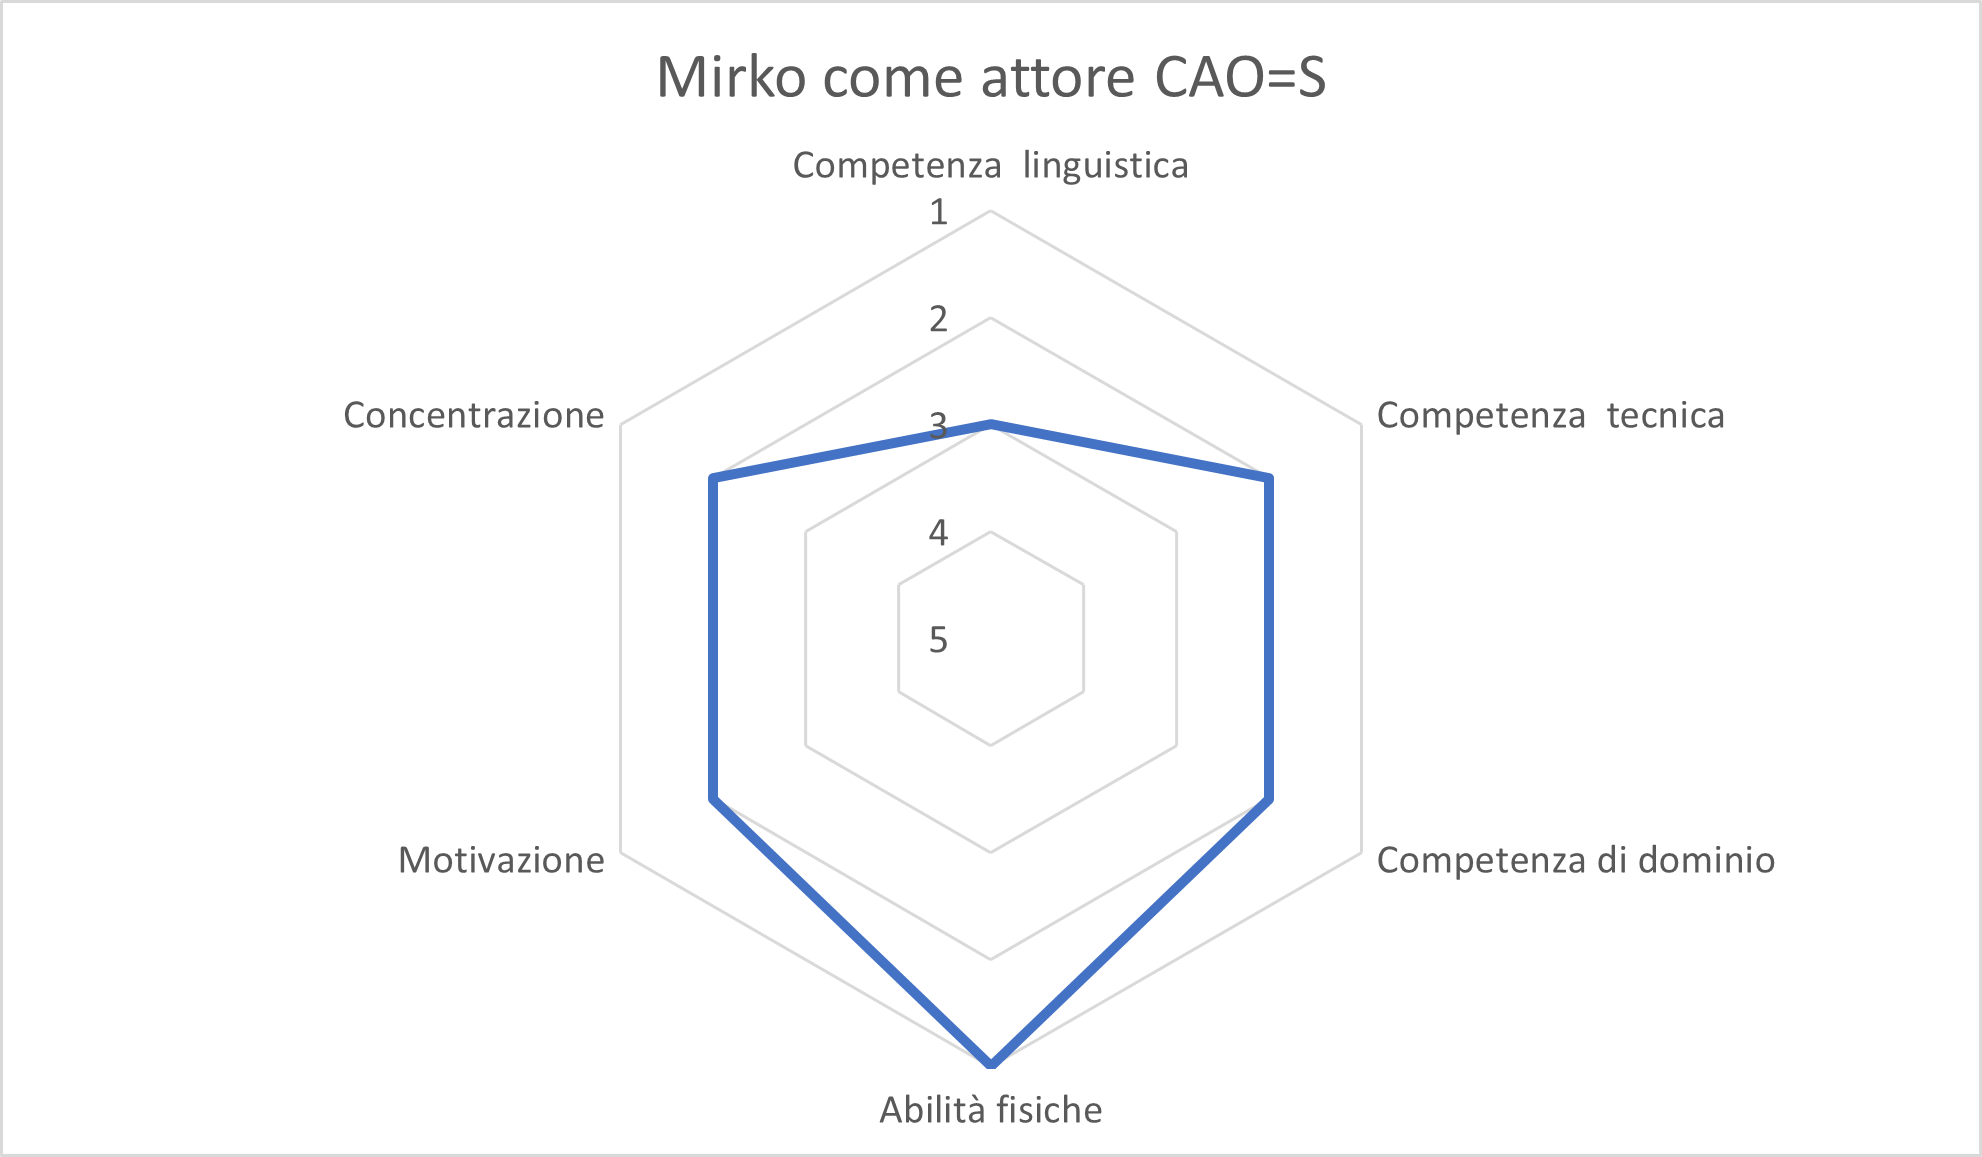
\includegraphics[height=8cm]{MirkoCAOS.png}
        \centering
    \end{figure}
    \begin{figure}[H]
        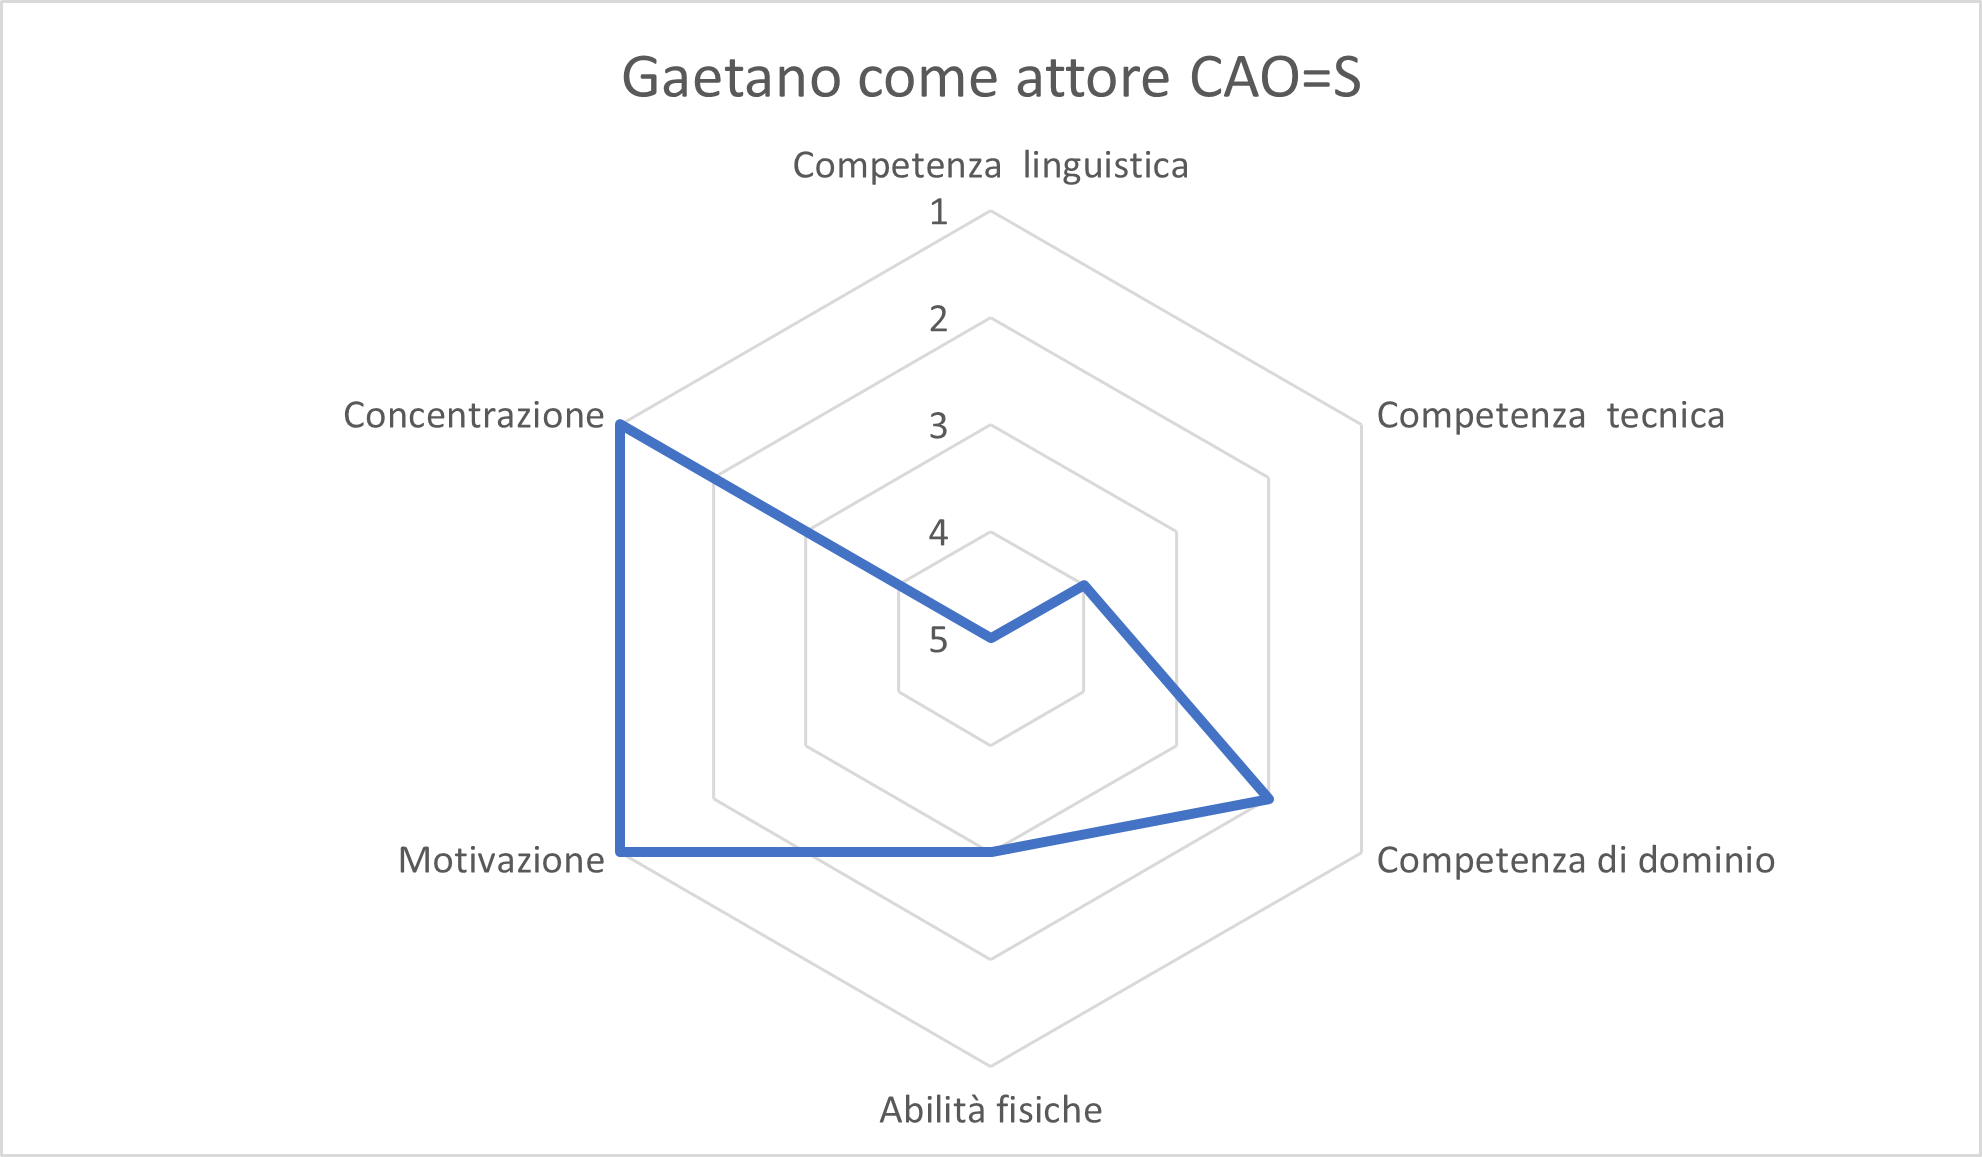
\includegraphics[height=8cm]{GaetanoCAOS.png}
        \centering
    \end{figure}
    \begin{figure}[H]
        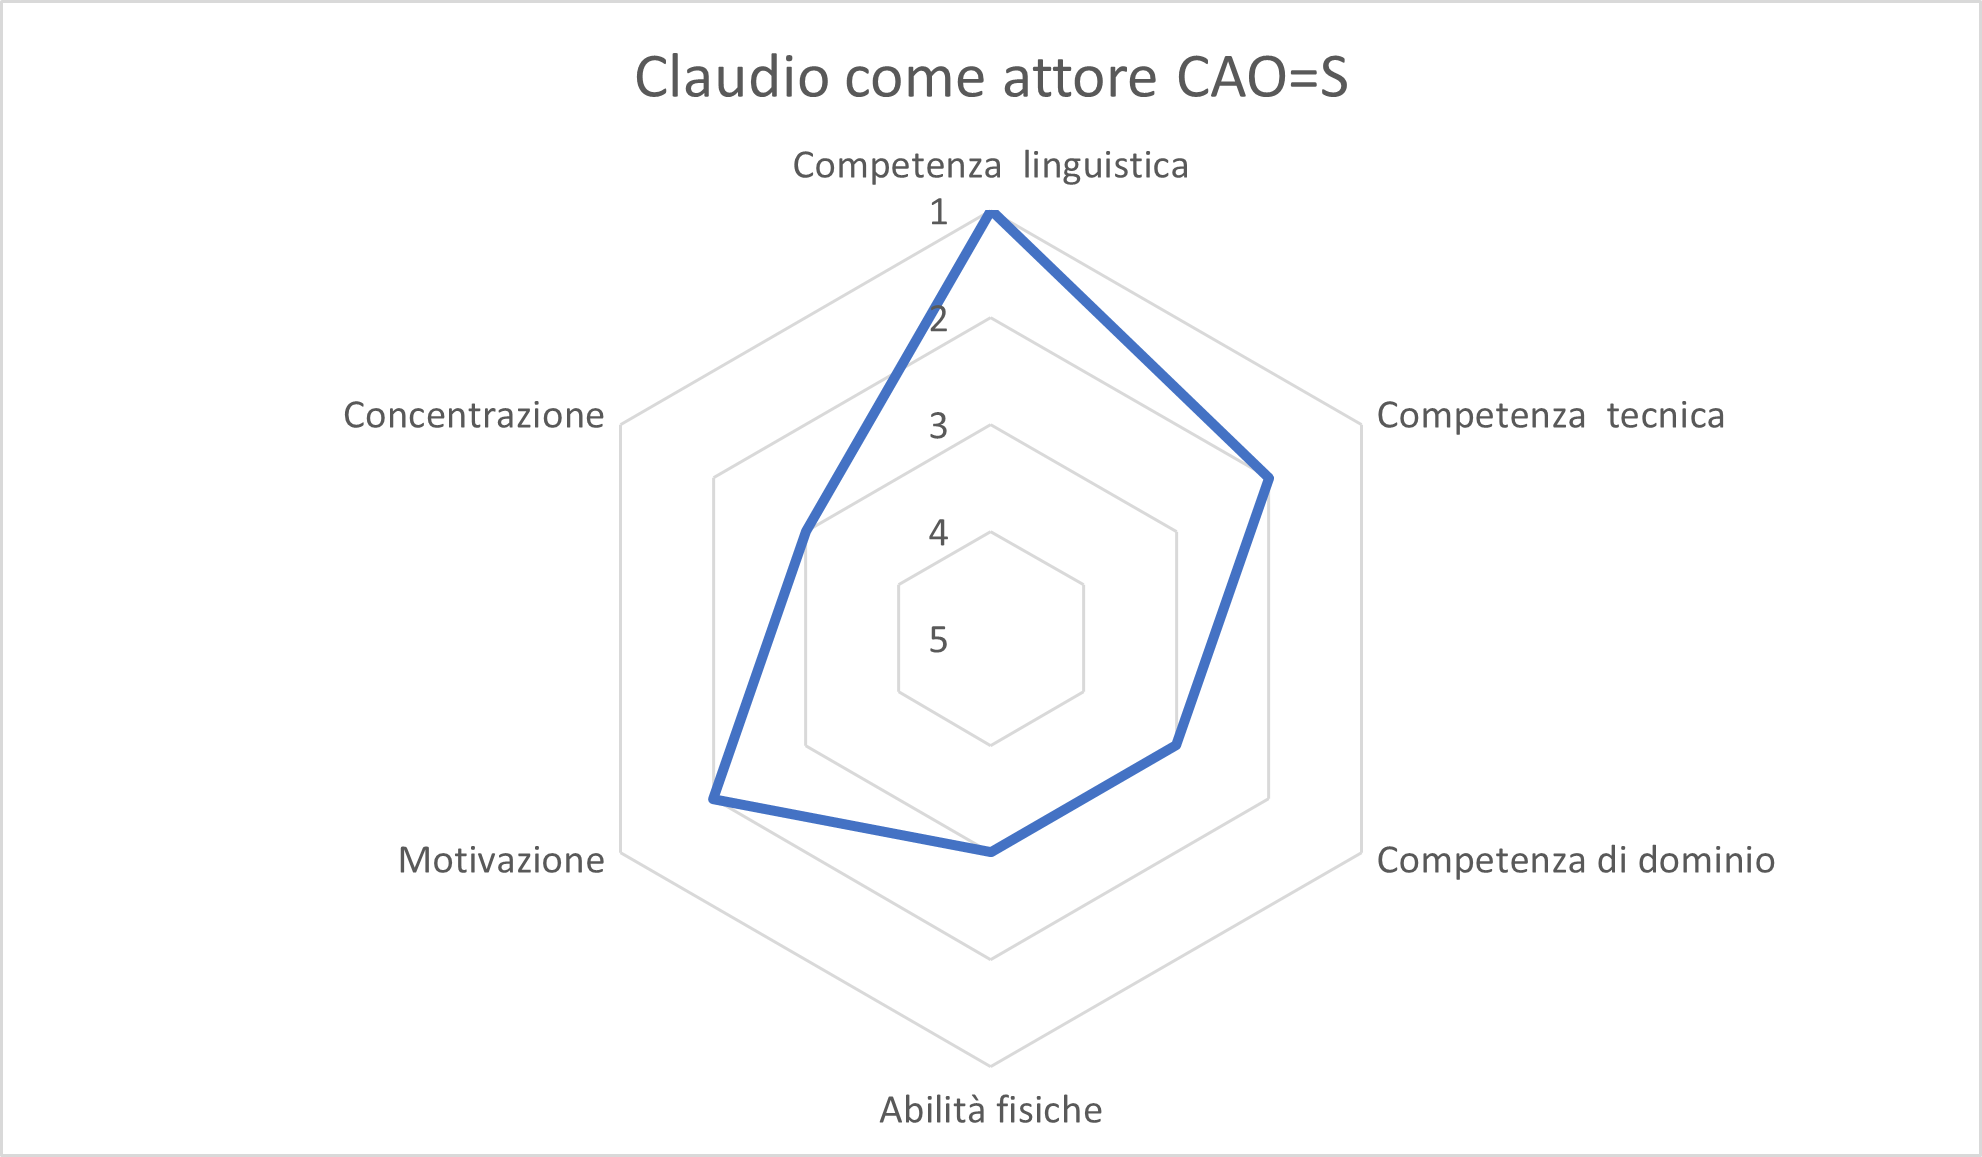
\includegraphics[height=8cm]{ClaudioCAOS.png}
        \centering
    \end{figure}
    \begin{figure}[H]
        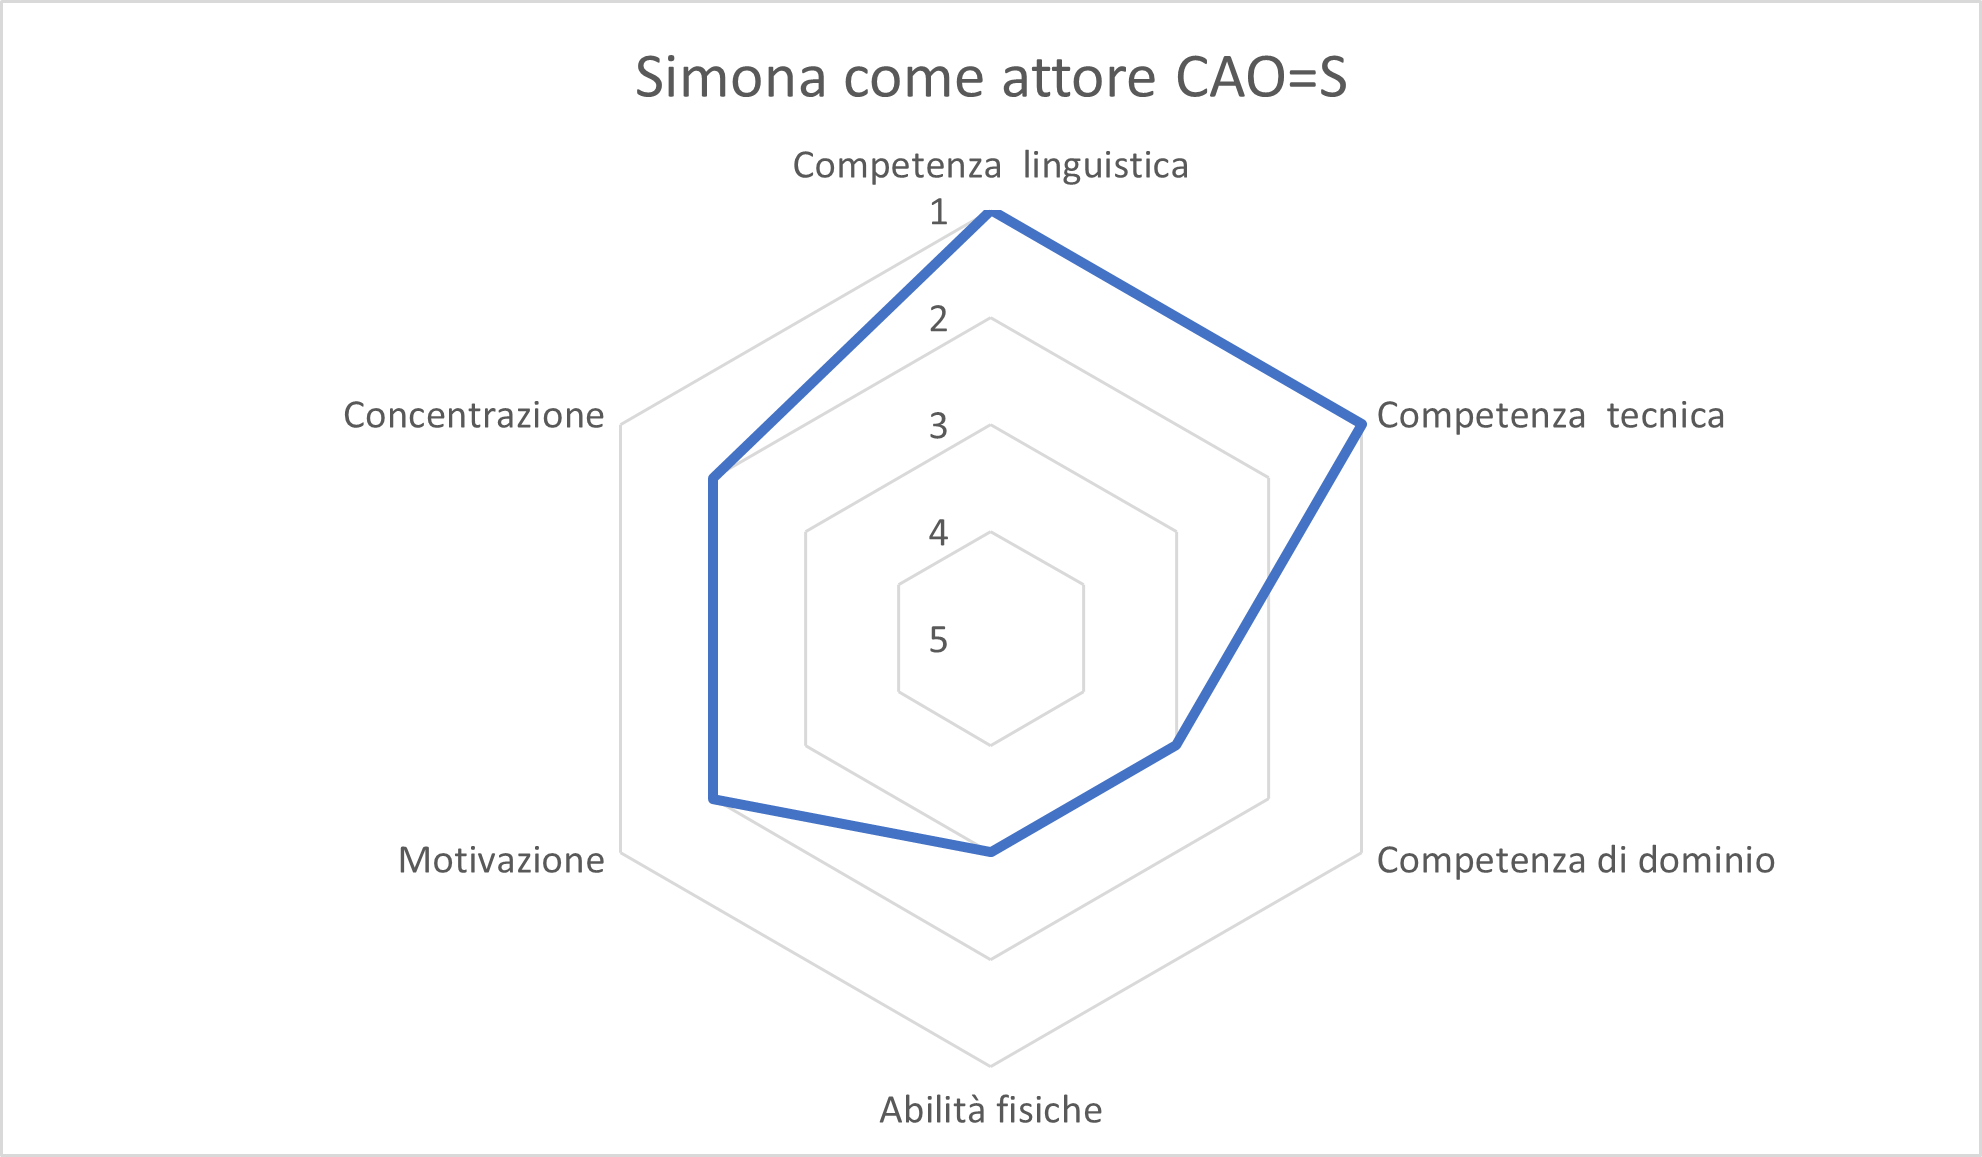
\includegraphics[height=8cm]{SimonaCAOS.png}
        \centering
    \end{figure}

    \subsection{Operazioni}
    Nel modello CAO=S le operazioni si basano su un modello CRUD, ovvero:
    \begin{itemize}
        \item Create
        \item Read
        \item Update
        \item Delete
    \end{itemize}
    Le singole operazioni compiute dai singoli attori sui singoli concetti vengono inserite in una tabella, che rappresenta, per ciascun attore, i tipi di operazione e i concetti. I nostri attori sono l'utente finale (il giocatore) e il supervisore, quindi dobbiamo fornire due tabelle. La prima è quella del giocatore:

    \begin{table}[H]
        \begin{tabularx}{\textwidth}{|c|c|c|c|c|}
        %\begin{tabular}{|c|c|c|c|c|}
            \hline
            \textbf{CONCEPT} & \textbf{CREATE} & \textbf{READ} & \textbf{UPDATE} & \textbf{DELETE} \\
            \hline
            \textbf{Account} & \cellcolor{gray} & \cellcolor{gray} & \cellcolor{gray} & \cellcolor{gray}\\
            \hline
            \textbf{Giochi} & \cellcolor{red} & \cellcolor{green} & \cellcolor{red} & \cellcolor{red} \\
            \hline
            \textbf{Commento} & \cellcolor{gray} & \cellcolor{gray} & \cellcolor{gray} & \cellcolor{gray} \\
            \hline
            \textbf{Categoria} & \cellcolor{red} & \cellcolor{green} & \cellcolor{red} & \cellcolor{red} \\
            \hline
            \textbf{Menu} & \cellcolor{red} & \cellcolor{green} & \cellcolor{red} & \cellcolor{red} \\
            \hline
            \textbf{Filtro} & \cellcolor{red} & \cellcolor{green} & \cellcolor{green} & \cellcolor{red} \\
            \hline
            \textbf{Amici} & \cellcolor{gray} & \cellcolor{gray} & \cellcolor{red} & \cellcolor{gray} \\
            \hline
            \textbf{Descrizione} & \cellcolor{red} & \cellcolor{gray} & \cellcolor{red} & \cellcolor{red} \\
            \hline
            \textbf{Preferiti} & \cellcolor{red} & \cellcolor{gray} & \cellcolor{red} & \cellcolor{red} \\
            \hline
            \textbf{FAQ} & \cellcolor{gray} & \cellcolor{green} & \cellcolor{red} & \cellcolor{gray} \\
            \hline
            \textbf{Parental Control} & \cellcolor{red} & \cellcolor{red} & \cellcolor{red} & \cellcolor{red} \\
            \hline
        %\end{tabular}
        \end{tabularx}
        \caption{\label{tab:giocatore}Tabella del giocatore.}
    \end{table}



    Di seguito mostriamo la tabella del supervisore, fondamentalmente identica alla precedente con la sola differenza nel concetto del Parental Control:

    \begin{table}[H]
        \begin{tabular}{|c|c|c|c|c|}
            \hline
            \textbf{CONCEPT} & \textbf{CREATE} & \textbf{READ} & \textbf{UPDATE} & \textbf{DELETE} \\
            \hline
            ... & ... & ... & ... & ... \\
            \hline
            \textbf{Parental Control} & \cellcolor{green} & \cellcolor{green} & \cellcolor{green} & \cellcolor{green} \\
            \hline
        \end{tabular}
        \caption{\label{tab:supervisore}Tabella del supervisore}
    \end{table}
    
    \subsubsection{Note}
    In questa prospettiva, creare significa che l’utente, attraverso il sito, crea un qualcosa di nuovo (come un account o un commento), lo stesso vale per l’aggiornamento e l’eliminazione. La voce “Read” sta ad indicare tutto ciò che l’utente può osservare di quel determinato concetto e il tipo di vista che l'utente ha su quel concetto. In rosso vengono messe tutte quelle operazioni che vengono eseguite da Gioco.it e l’utente non può intervenire in alcun modo. In grigio tutte le operazioni già presenti nel sito, che non hanno subito modifiche dopo la nostra progettazione. In verde le nostre modifiche apportate al sito.

    \section{Progettazione dell'interazione}
    In questa sezione definiremo l'architettura dell'informazione che abbiamo definito nella sezione \ref{section:architettura dell'informazione} e nelle viste CAO=S (sezione \ref{section:CAOS}), prima proponendo dei Blueprints, uno schema in cui viene spiegato il modello concettuale del sito, e successivamente proporremo i Wireframes, delle rappresentazioni delle schermate principali del sito.

    \subsection{Homepage}
    La homepage dovrà essere più coerente e ordinata rispetto all'attuale design, più orientato alla minimizzazione del carico cognitivo dell'utente. Il nuovo design dovrà permettere sia di trovare giochi nuovi e sia di presentare giochi utilizzati di frequente. Inoltre, essa dovrà mostrare tutte le funzionalità messe a disposizione del sito (es: categorie, account, ecc).

    \subsubsection{Header}
    Essa permetterà di ricercare i giochi per nome, visualizzare le categorie, visualizzare il proprio account e avrà il logo per tornare alla homepage. A differenza del vecchio design permetterà di visualizzare tutte le categorie e non soltanto alcune. 

    \subsubsection{Footer}
    Esso conterrà le informazioni dell'azienda, assistenza clienti (FAQ) e la possibilità di cambiare la lingua. Il design rimarrà pressoché lo stesso.
    
    \subsection{Card del gioco}
    Nella versione attuale le card dei giochi non contengono informazione rilevanti per i supervisori, infatti nel nuovo design saranno presenti dei simboli che descrivono i contenuti del gioco (es: limiti di età, violenza, presenza di armi, ecc).

    \subsection{Gioco}
    La schermata del gioco dovrà contenere gli stessi elementi che contiene attualmente. Sarà necessario quindi un riquadro per la visualizzazione del gioco e la sua descrizione. Saranno presenti i comandi che permettono di andare direttamente a mettere nei preferiti un gioco e a spostarsi nella sezione commenti. Poichè come detto nella sezione di Inspezione \ref{} è presente dell'inutile spazio vuoto alla destra dei giochi il nostro redesign andrà ad occupare lo spazio lasciato vuoto, riempiendolo per quanto possibile con la schermata di gioco. Sarà anche importante mantenere la sezione legata al supporto e alla spiegazione del gioco (precedentemente erroneamente chiamata "Soluzione").

    \section{Blueprints}

\end{document}